
\RequirePackage{currfile} 

\documentclass{beamer}

\definecolor{rougeb}{rgb}{0.75,0.01,0}

%\setbeamercolor{subsection in toc}{fg=red} %change la couleur de la ToC
\setbeamerfont{section number projected}{family=\rmfamily,series=\bfseries,size=\normalsize}
\setbeamercolor{section number projected}{bg=rougeb,fg=white}
\setbeamerfont{subsection number projected}{family=\rmfamily,series=\bfseries,size=\normalsize}
\setbeamercolor{subsection number projected}{bg=rougeb,fg=white}

%%%%%%%%%%%%%%%%%%%%%%%%%%%%%%%%%%%%%%%%%
% Beamer Presentation
% LaTeX Template
% Version 1.0 (10/11/12)
%
% This template has been downloaded from:
% http://www.LaTeXTemplates.com
%
% License:
% CC BY-NC-SA 3.0 (http://creativecommons.org/licenses/by-nc-sa/3.0/)
%
%%%%%%%%%%%%%%%%%%%%%%%%%%%%%%%%%%%%%%%%%

%----------------------------------------------------------------------------------------
%	PACKAGES AND THEMES
%----------------------------------------------------------------------------------------




\mode<presentation> {

% The Beamer class comes with a number of default slide themes
% which change the colors and layouts of slides. Below this is a list
% of all the themes, uncomment each in turn to see what they look like.

%\usetheme{default}
%\usetheme{AnnArbor}
%\usetheme{Antibes} %pas mal du tout
%\usetheme{Bergen}
%\usetheme{Berkeley}
\usetheme{Berlin} %vraiment excellent -----------------------
%\usetheme{Boadilla}
%\usetheme{CambridgeUS} %bien --> light
%\usetheme{Copenhagen} % bien : ressemble à warsaw
%\usetheme{Darmstadt} %tres tres bien
%\usetheme{Dresden} %excellent (berlin avce la ToC modifiée) --------
%\usetheme{Frankfurt} %bien
%\usetheme{Goettingen}
%\usetheme{Hannover}
%\usetheme{Ilmenau} %excellent (berlin avce la ToC modifiée) --------
%\usetheme{JuanLesPins} % stylé mais peu fonctionnel
%\usetheme{Luebeck} % bien : ressemble à warsaw
%\usetheme{Madrid} % bof
%\usetheme{Malmoe} %\usetheme{Luebeck} % bien : ressemble à warsaw
%\usetheme{Marburg}
%\usetheme{Montpellier} %pas mal du tout ressemble a antibes
%\usetheme{PaloAlto}
%\usetheme{Pittsburgh}
%\usetheme{Rochester}
%\usetheme{Singapore} % berlin en bcp moins bien
%\usetheme{Szeged} %excellent (berlin avce la footer modifié) --------
%\usetheme{Warsaw} %bien

% As well as themes, the Beamer class has a number of color themes
% for any slide theme. Uncomment each of these in turn to see how it
% changes the colors of your current slide theme.

%\usecolortheme{albatross}
\usecolortheme{beaver}
%\usecolortheme{beetle}
%\usecolortheme{crane}
%\usecolortheme{dolphin}
%\usecolortheme{dove}
%\usecolortheme{fly}
%\usecolortheme{lily}
%\usecolortheme{orchid}
%\usecolortheme{rose}
%\usecolortheme{seagull}
%\usecolortheme{seahorse}
%\usecolortheme{whale}
%\usecolortheme{wolverine}

%\setbeamertemplate{footline} % To remove the footer line in all slides uncomment this line
%\setbeamertemplate{footline}[frame number] % To replace the footer line in all slides with a simple slide count uncomment this line

%\setbeamertemplate{navigation symbols}{} % To remove the navigation symbols from the bottom of all slides uncomment this line

\setbeamercovered{transparent} % Fait apparaître les animations en grisé (utile pour la conception, mais peut être commenté lors de la remise du document final)

% Pour utiliser une police à empattements partout
\usefonttheme{serif}

% Pour rajouter la numérotation des frames dans les pieds de page
\newcommand*\oldmacro{}%
\let\oldmacro\insertshorttitle%
\renewcommand*\insertshorttitle{%
  \oldmacro\hfill%
  \insertframenumber\,/\,\inserttotalframenumber}

}

\usepackage{graphicx} % Allows including images
\usepackage{booktabs} % Allows the use of \toprule, \midrule and \bottomrule in tables

% Les autres packages utiles  notamment pour le français, les accents ou Python
\usepackage{natbib}         % Pour la bibliographie
\usepackage{url}            % Pour citer les adresses web
\usepackage[T1]{fontenc}    % Encodage des accents
\usepackage[utf8]{inputenc} % Lui aussi
\usepackage[frenchb]{babel} % Pour la traduction française
\usepackage{numprint}       % Histoire que les chiffres soient bien

\usepackage{amsmath}        % La base pour les maths
\usepackage{mathrsfs}       % Quelques symboles supplémentaires
\usepackage{amssymb}        % encore des symboles.
\usepackage{amsfonts}       % Des fontes, eg pour \mathbb.

\usepackage{cancel}

%\usepackage[svgnames]{xcolor} % De la couleur

%%% Si jamais vous voulez changer de police: décommentez les trois 
%\usepackage{tgpagella}
%\usepackage{tgadventor}
%\usepackage{inconsolata}

%%% Pour L'utilisation de Python
\usepackage{minted}
\usemintedstyle{friendly}

\usepackage{graphicx} % inclusion des graphiques
\usepackage{wrapfig}  % Dessins dans le texte.

\usepackage{tikz}     % Un package pour les dessins (utilisé pour l'environnement {code})
\usepackage[demo]{tikzpeople}
\usepackage[framemethod=TikZ]{mdframed}
\usepackage{chronosys}

% Les macros et raccourcis personnels
% Ce fichier contient toutes les macros que vous pouvez avoir envie de définir 
% si vous les utilisez plusieurs fois dans le document.

\PassOptionsToPackage{svgnames}{color}

% Un environnement pour bien présenter le code informatique
\newenvironment{code}{%
\begin{mdframed}[linecolor=green,innerrightmargin=30pt,innerleftmargin=30pt,
backgroundcolor=black!5,
skipabove=10pt,skipbelow=10pt,roundcorner=5pt,
splitbottomskip=6pt,splittopskip=12pt]
}{%
\end{mdframed}
}

% Un raccourci pour composer les unités correctement (en droit)
% Exemple: $v = 10\U{m.s^{-1}}$
\newcommand{\U}[1]{~\mathrm{#1}}

% Les guillemets \ofg{par exemple}
\newcommand{\ofg}[1]{\og{}#1\fg{}}

% Le d des dérivées doit être droit: \frac{\dd x}{\dd t}
\newcommand{\dd}{\text{d}}

% La dérivée temporelle, tellement courante en physique, avec les d droits
\newcommand{\ddt}[1]{\frac{\dd #1}{\dd t}}

% Des parenthèses, crochets et accolades qui s'adaptent automatiquement à la 
% taille de ce qu'il y a dedans
\newcommand{\pa}[1]{\left(#1\right)}
\newcommand{\pac}[1]{\left[#1\right]}
\newcommand{\paa}[1]{\left\{#1\right\}}

% Un raccourci pour écrire une constante
\newcommand{\cte}{\text{C}^{\text{te}}}

% Pour faire des indices en mode texte (comme les énergie potentielles)
\newcommand{\e}[1]{_{\text{#1}}}

% Le produit vectoriel a un nom bizarre:
\newcommand{\vectoriel}{\wedge}

% On définit le titre et l'auteur du document

\title[Cryptographie homomorphe]{Étude et implémentation d'un schéma de chiffrement homomorphe}
\author{Milan \textsc{Gonzalez-Thauvin}}
\institute[ ]{Thème : Transport}
\date{TIPE session 2019}

% On démarre le document proprement dit
\begin{document}

% Rien d'autre à faire qu'afficher le titre
\begin{frame}
\titlepage 
\end{frame}


% La table des matières utilise ce que vous donnez aux commandes \section et 
% \subsection tout au long de la présentation.
\begin{frame}
\frametitle{Plan de l'exposé} 
\tableofcontents 
\end{frame}

% Introduction
\addtocontents{toc}{\protect\setcounter{tocdepth}{2}}
%La ligne ci dessus permet de masquer les subsections de l'intro dans la ToC

\section{Introduction}

\subsection{La Cryptographie}

\begin{frame}
\frametitle{Introduction}
    \begin{tikzpicture}[pin distance=1cm,every pin/.append style={font=\sffamily\itshape}]
    \node[alice,minimum size=2cm,pin={[text width=2em]40:{$\operatorname{enc}$}}] (A) at (2,2) {Alice};
    \node[bob,mirrored, minimum size=2cm,pin={[text width=2em]140:{$\operatorname{dec}$}}] (B) at (10,2) {Bob};
    \node[criminal,female,minimum size=2cm] at (6,-0.5) {Eve};
    \draw [thick,->] (A) -- (B) node[midway,above] {Message secret};
    \end{tikzpicture}
\end{frame}

\begin{frame}{Histoire}
    \startchronology[startyear=1910,stopyear=2019,color=gray,height=7ex,width=\hsize,startdate=false, stopdate=false]
    \chronoperiodecoloralternation{brown,rougeb}
    \chronoperiode[startdate=false, stopdate=false]{1910}{1950}{Cryptographie symétrique}
    \chronoperiode[stopdate=false]{1950}{2019}{Cryptographie asymétrique}
    \chronoevent[markdepth=25pt]{1978}{Invention du RSA}
    \chronoevent[markdepth=50pt]{2009}{Thèse de Craig Gentry}
    \stopchronology
\end{frame}

\subsection{La Cryptographie homomorphe}

\begin{frame}
\frametitle{La cryptographie homomorphe}

\begin{figure}
\begin{tikzpicture}

\node[alice, minimum size=2.1cm, xshift=-1.5cm] at (0, 2) {Alice};

\draw [->] (0, 2) -- (4,2);
\node [above] at (2,2) {Entrées chiffrées};

\draw [->] (4,1) -- (0,1);
\node [below] at (2,1) {Résultat chiffré};

\node[bob, monitor, mirrored, minimum size=2.1cm, xshift=1.75cm] at (5, 2) {Bob};
\node [above] at (6,4) {Gros calculs};

\end{tikzpicture}
\end{figure}

\end{frame}

\begin{frame}{La cryptographie homomorphe}

\begin{alertblock}{Définition : Calculer sur des chiffrés}
Si $m$ est un mot \textbf{clair}, $c = \operatorname{enc}(m)$ son \textbf{chiffré}, et $f$ une fonction, $f$ est \textbf{compatible} pour le schéma si
    $$\operatorname{dec}(f(c)) = f(m)$$
\end{alertblock}

\begin{alertblock}{En pratique} % Bloc alerte rouge
\textbf{Somme} et \textbf{produit} car \textbf{polynôme}
\end{alertblock}
    
\end{frame}

\begin{frame}{La cryptographie homomorphe}

\begin{alertblock}{Définition : Cryptographie partiellement homomorphe}
On peut effectuer des additions \textbf{et/ou} des multiplications en nombre \textbf{fini}
\end{alertblock}

\begin{alertblock}{Définition : Cryptographie complètement homomorphe}
On peut effectuer des additions \textbf{et} des multiplications en nombre \textbf{infini} 
\end{alertblock}

\begin{alertblock}{Pourquoi fait on la distinction ?}
La cryptographie homomorphe se base sur du \textbf{bruit}.
\end{alertblock}

\end{frame}

\begin{frame}{La cryptographie homomorphe}
    \begin{center}
    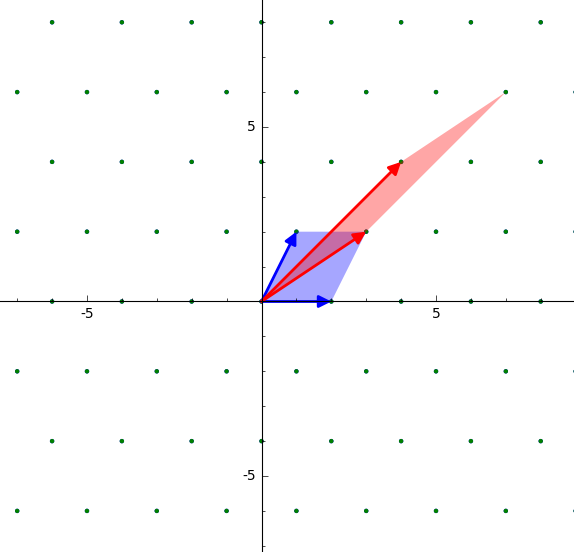
\includegraphics[scale=0.43]{images/exemple_reseau2.png} 
    \end{center}
\end{frame}{}

\begin{frame}{État de l'art}
    \begin{alertblock}{Avant la Thèse de Craig Gentry}
    Cryptographie \textbf{partiellement homomorphe}
    \end{alertblock}
    \begin{alertblock}{Thèse de Craig Gentry (2009)}
    Astuce : \textbf{bootstrap}
    \end{alertblock}
    \begin{alertblock}{Depuis la thèse de Craig Gentry}
        Beaucoup de schémas \textbf{théoriques}\\
        Aucune application concrète car \textbf{aucun n'est assez performant}
    \end{alertblock}{}
\end{frame}{}


\addtocontents{toc}{\protect\setcounter{tocdepth}{2}}

%fin de l'introduction : rajouter le schéma va-et-vient  + finir l'etat de l'art

% Schéma
\section{Le schéma de Damien sthelé}

% essayer de faire une diapositive de début de partie 

\subsection{Partie théorique}

\begin{frame}{Principe mathématique}
	\begin{block}{Le schéma de Damien Sthélé : Cryptographie sur les entiers}
		clef privée : $ sk = p $ 
		clef publique : $ pk = x_1, \cdots , x_r / \forall i \in [ 1,r ], x_i \leftarrow p q_i + r_i $
		avec $ x_0 $ le plus grand et $ \frac{x_1}{2} $ impair. %ajouter partie entiere
	\end{block}

\end{frame}

\begin{frame}
\frametitle{Principe}
\framesubtitle{La théorie}
\end{frame}


\begin{frame}
\frametitle{Les fonctions}
\framesubtitle{add, mul}
\end{frame}

% Implémentation
\subsection{Implémentation}

\begin{frame}
\frametitle{Fonctions de base}
\framesubtitle{enc, dec}
\end{frame}



\begin{frame}
\frametitle{Le bootstrap}
\end{frame}

% Améliorations
\section{Améliorations}

\subsection{Surcouche}

\begin{frame}
\frametitle{Surcouche}
\end{frame}

\subsection{Performances}

\begin{frame}
\frametitle{Paramètres}
\end{frame}

\subsection{Sécurité}

\begin{frame}
\frametitle{Génération des clefs}
\end{frame}

% Application
\section{Application}

\subsection{Contexte}

\begin{frame}
\frametitle{Contexte}
\end{frame}

\begin{frame}
\frametitle{Mise en forme}
\end{frame}

\subsection{Résultats}

\begin{frame} %Utile ?
\frametitle{Fonctionne ?}
\end{frame}

\begin{frame}
\frametitle{Performance}
\end{frame}

\begin{frame}
\frametitle{Sécurité}
\end{frame}

\section{Conclusion}

\begin{frame}
\frametitle{Conclusion}
\end{frame}

\end{document}
